%%%%%%%%%%%%%%%%%%%%%%%%%%%%%%%%%%%%%%%%%%%%%%%%%%%%%%%%%%%%%%%%%%%%%%%%%%%%
% AGUtmpl.tex: this template file is for articles formatted with LaTeX2e,
% Modified March 2013
%
% This template includes commands and instructions
% given in the order necessary to produce a final output that will
% satisfy AGU requirements.
%
% PLEASE DO NOT USE YOUR OWN MACROS
% DO NOT USE \newcommand, \renewcommand, or \def.
%
% FOR FIGURES, DO NOT USE \psfrag or \subfigure.
%
%%%%%%%%%%%%%%%%%%%%%%%%%%%%%%%%%%%%%%%%%%%%%%%%%%%%%%%%%%%%%%%%%%%%%%%%%%%%
%
% All questions should be e-mailed to latex@agu.org.
%
%%%%%%%%%%%%%%%%%%%%%%%%%%%%%%%%%%%%%%%%%%%%%%%%%%%%%%%%%%%%%%%%%%%%%%%%%%%%
%
% Step 1: Set the \documentclass
%
% There are two options for article format: two column (default)
% and draft.
%
% PLEASE USE THE DRAFT OPTION TO SUBMIT YOUR PAPERS.
% The draft option produces double spaced output.
%
% Choose the journal abbreviation for the journal you are
% submitting to:

% jgrga JOURNAL OF GEOPHYSICAL RESEARCH
% gbc   GLOBAL BIOCHEMICAL CYCLES
% grl   GEOPHYSICAL RESEARCH LETTERS
% pal   PALEOCEANOGRAPHY
% ras   RADIO SCIENCE
% rog   REVIEWS OF GEOPHYSICS
% tec   TECTONICS
% wrr   WATER RESOURCES RESEARCH
% gc    GEOCHEMISTRY, GEOPHYSICS, GEOSYSTEMS
% sw    SPACE WEATHER
% ms    JAMES
%
%
%
% (If you are submitting to a journal other than jgrga,
% substitute the initials of the journal for "jgrga" below.)

\documentclass[draft,jgrga]{agutex}
%\documentclass[jgrga]{agutex}

% To create numbered lines:

% If you don't already have lineno.sty, you can download it from
% http://www.ctan.org/tex-archive/macros/latex/contrib/ednotes/
% (or search the internet for lineno.sty ctan), available at TeX Archive Network (CTAN).
% Take care that you always use the latest version.

% To activate the commands, uncomment \usepackage{lineno}
% and \linenumbers*[1]command, below:

 \usepackage{lineno}
% \linenumbers*[1]

%  To add line numbers to lines with equations:
%  \begin{linenomath*}
%  \begin{equation}
%  \end{equation}
%  \end{linenomath*}
%%%%%%%%%%%%%%%%%%%%%%%%%%%%%%%%%%%%%%%%%%%%%%%%%%%%%%%%%%%%%%%%%%%%%%%%%
% Figures and Tables
%
%
% DO NOT USE \psfrag or \subfigure commands.
%
%  Figures and tables should be placed AT THE END OF THE ARTICLE,
%  after the references.
%
%  Uncomment the following command to include .eps files
%  (comment out this line for draft format):
  \usepackage[dvips]{graphicx}
%
%  Uncomment the following command to allow illustrations to print
%   when using Draft:
  \setkeys{Gin}{draft=false}
%
% Substitute one of the following for [dvips] above
% if you are using a different driver program and want to
% proof your illustrations on your machine:
%
% [xdvi], [dvipdf], [dvipsone], [dviwindo], [emtex], [dviwin],
% [pctexps],  [pctexwin],  [pctexhp],  [pctex32], [truetex], [tcidvi],
% [oztex], [textures]
%
% See how to enter figures and tables at the end of the article, after
% references.
%
%  Other packages:
\usepackage{amsmath}
\usepackage[usenames]{color}
\usepackage{ulem}
\usepackage{url}
\usepackage{lscape}
%\usepackage[pdftex]{graphicx}
%\usepackage{epstopdf}
%\usepackage{pgfplots}
\usepackage{stmaryrd}
\usepackage{soul}		% this package allows  highlighting -- useful in the text

%
%
%% ------------------------------------------------------------------------ %%
%
%  ENTER PREAMBLE
%
%% ------------------------------------------------------------------------ %%

% Author names in capital letters:
\authorrunninghead{NEEF ET AL.}

% Shorter version of title entered in capital letters:
\titlerunninghead{ANGULAR MOMENTUM ASSIMILATION}

%Corresponding author mailing address and e-mail address:
\authoraddr{Corresponding author: L.J. Neef,
%Helmholtz -Zentrum f{\"u}r Ozeanforschung (GEOMAR),
D{\"u}sternbrooker Weg 20,
D-24105 Kiel, Germany
(neef@geomar.de)}

\begin{document}
\bibliographystyle{agu08}

%% ------------------------------------------------------------------------ %%
%
%  TITLE
%
%% ------------------------------------------------------------------------ %%


\title{Earth Rotation Parameters in Atmospheric Data Assimilation}
%
% e.g., \title{Terrestrial ring current:
% Origin, formation, and decay $\alpha\beta\Gamma\Delta$}
%

%% ------------------------------------------------------------------------ %%
%
%  AUTHORS AND AFFILIATIONS
%
%% ------------------------------------------------------------------------ %%


%Use \author{\altaffilmark{}} and \altaffiltext{}

% \altaffilmark will produce footnote;
% matching \altaffiltext will appear at bottom of page.

 \authors{Lisa Neef\altaffilmark{1}, 
Katja Matthes \altaffilmark{1,2}, 
Kevin Raeder \altaffilmark{3}, 
Sebastian Wahl \altaffilmark{1}, and
Nick Pedatella \altaffilmark{4}
}

\altaffiltext{1}{Ocean Circulation and Climate Dynamics - Marine Meteorology,
   GEOMAR Helmholtz Centre for Ocean Research Kiel, Kiel, Germany.}
\altaffiltext{2}{Christian-Albrechts Universit\"at zu Kiel, Kiel, Germany.}
\altaffiltext{3}{Institute for Mathematics Applied to Geosciences, 
National Center for Atmospheric Research, Boulder, Colorado, USA.}
\altaffiltext{4}{COSMIC Program Office, University Corporation for Atmospheric Research, Boulder, Colorado, USA.}


%% ------------------------------------------------------------------------ %%
%
%  ABSTRACT
%
%% ------------------------------------------------------------------------ %%

% >> Do NOT include any \begin...\end commands withinA
% >> the body of the abstract.

\begin{abstract}
% (A) the global AM of the atmosphere is observed at high accuracy in terms of ERPs, which has led to suggestions that it can be assimilated into atmo/ocean models in order to remove biases and add extra information. 
Variations in the atmosphere's angular momentum are observed consistently and at high accuracy in terms of variations in the Earth's rate of rotation and polar orientation.
It has been suggested that these Earth rotation parameters could therefore be assimilated into atmosphere or ocean models in order to add extra information, either when conventional observations are sparse, or in addition.
%
% (B) But the AM also represents global integrals of the wind and pressure fields, and it is unclear how the information from such an observation would be distributed as a correction over the model variable fields.
However, the atmospheric angular momentum represents represents global integrals of the wind and pressure fields, and it is unclear how a data assimilation system would distribute the information from such observations across model variable fields.  
%
% (T) For this reason we ran idealized DA experiments wherein ERP observations are assimilated into the CAM, but with and without local temperature observations. We found that it really doesn't work, but that AAM-space comparison of the different simulations makes the different constrains imposed in each case clear, so we use WACCM simulations with real data assimilations to show that ERPs make a useful parameter for evaluating ensemble reliability in a DA system.  
To test this, we perform idealized assimilation experiments with the Community Atmosphere Model (CAM) within the Data Assimilation Research Testbed (DART), assimilating atmospheric angular momentum observations both in the presence and absence of local temperature observations. 
The experiments show that
assimilating the atmospheric angular momentum suffers from a high sampling error relative to a very small state-to-observation covariances, and therefore
generally leads to filter divergence.
Nevertheless, comparing the experiments in terms of their angular momentum also illustrates the different constraints imposed in each case. 
This suggests that the Earth rotation parameters can be used as a tool to evaluate ensemble reliability and accuracy of a data assimilation system, without being assimilated. 
We illustrate this idea with a set of ensemble simulations of the Whole Atmosphere Community Climate Model (WACCM).

\end{abstract}

%% ------------------------------------------------------------------------ %%
%
%  BEGIN ARTICLE
%
%% ------------------------------------------------------------------------ %%

% The body of the article must start with a \begin{article} command
%
% \end{article} must follow the references section, before the figures
%  and tables.

\begin{article}

%% ------------------------------------------------------------------------ %%
%
%  MATH ABBREVIATSIONS
%
%% ------------------------------------------------------------------------ %%
% note that AGU doesn't want us to use macros, so have to replace these manually
% later. 
\newcommand{\degree}{\ensuremath{^\circ}}
\newcommand{\WACCMNODA}{E1}
\newcommand{\WACCMTROPICS}{E2}
\newcommand{\WACCMGLOBAL}{E3}
%\newcommand{\NCARFULL}{E4}
\newcommand{\NODA}{E4}
\newcommand{\ERPALL}{E5}
\newcommand{\RST}{E6}
\newcommand{\ERPRST}{E7}


%% ------------------------------------------------------------------------ %%
%
%  TEXT
%
%% ------------------------------------------------------------------------ %%

\section{Introduction}
% much shorter attempt at the introduction

% P1: general knowledge: Earth rotation data contain info about the AM of the Earth system, but it's unclear how to use this info  
Variations in the rotation and orientation of the Earth are measured regularly and at high accuracy using space geodesy \citep{Gross1992,iers}. 
These measurements contain information about the atmosphere, oceans, and continental hydrosphere, which all exchange angular momentum with the solid Earth, thereby causing both the Earth's rate of rotation and its polar orientation to fluctuate. 

% P2: previous work and gaps in it: others have shown that certain model adjustments rectify diffs between observed ERPs and modeled AM, most notably Saynish -- but they did not show that this actually results in a better model
The atmosphere and ocean dominate sub-decadal Earth rotation variations. 
We can therefore potentially use the difference between the observed Earth rotation anomalies, and modeled atmospheric and oceanic angular momenta, to correct models of the atmosphere and oceans. 
Indeed, previous studies have used Earth rotation data to evaluate the accuracy of, 
and identify biases in, atmosphere models \citep{Boer1990, Rosen2000}, ocean 
models \citep{Gross1996a} or reanalyses \citep{Yu1999, Aoyama2000, 
Paek2012a,Berrisford2011},
%\citet{Ayoma2000} identified potential problems in reanalysis wind data due to discrepancies between predicted and observed LOD variations.
%\citet{Paek2012} used LOD observations to evaluate the accuracy of and identify biases in various reanalysis sets.
%\citet{Rosen2000} used observed LOD anomalies to evaluate the interannual variability simulated by AMIP models.
%\citet{Gross2006a} used observed polar motion to identify discrepancies in ocean tide models: [FILL IN]
%\citet{Berrisford2011} used the angular momentum / torque budget to compare ERA-Interim and ERA-40.  

\citet{Saynisch2010,Saynisch2011} and \citet{Saynisch2012} assimilated the residual between observed Earth rotation parameters and the estimated atmospheric angular momentum--the residual being an estimate of the oceanic angular momentum-- into two ocean models of varying complexity. 
Their simulations were able to close the Earth angular momentum budget by adjusting the modeled oceanic angular momentum, while simultaneously keeping the modeled ocean state in agreement with other ocean observations.  
\citet{Saynisch2010} and \citet{Saynisch2012} showed that the axial angular momentum budget is mainly closed by changing large-scale model parameters such as the freshwater flux, while \citet{Saynisch2011} found that closing the equatorial angular momentum budget in particular required changes in the model's current field. 

These results suggest that an atmosphere model could also benefit from the assimilation of Earth rotation observation, especially since the atmosphere dominates subdecadal length-of-day variations and accounts for at least half of subdecadal polar motion variations. 
Many large-atmospheric phenomena that dominate local weather but are subject to longer-timescale climate fluctuations, such as 
%the position and intensity of the storm tracks \hl{CITE}, 
sudden stratospheric warmings \citep{Neef2014} and the Madden Julian Oscillation \citep{Weickmann1992}, all have discernible footprints in Earth rotation anomalies. 
Climate reanalyses, while heavily constrained by observations from the surface to the lower stratosphere, still have discrepancies in the atmosphere's angular momentum budget \citep{Berrisford2011,Lehmann2012}, and  may therefore benefit from adding atmosphere angular momentum to the assimilated observations. 

However, the studies of \citet{Saynisch2010,Saynisch2011} and \citet{Saynisch2012} also faced a major challenge in that they attempted to constrain large, global model fields with observations of three global parameters, which presents a strongly underconstrained optimization problem. 
While these studies found that reconciling a model to observed Earth rotation variations leads to physically interesting and plausible adjustments to the model fields, the solutions found by the data assimilation in these simulations may not have been unique or truly closer to the true state of the ocean.  

% P3: how our study closes the gap: We show how a model state is updated using obseved ER information and identif the problems thereing, using (1) idealized experiments where the true error is known, and (2) a comparison to more conventional obs.
This study examines the potential of observed Earth rotation variations to (Section \ref{sec:evaluation_variable}) serve as a tool to evaluate data assimilation systems, and (Section \ref{sec:assimilation_variable}) constrain an atmosphere model as an assimilated variable.
% P4: Organization of the paper
Section \ref{sec:methods} describes the data assimilation experiments, observations assimilated, assimilation method, and models used.
The results are summarized and discussed in Section \ref{sec:discussion}.



%-------------------------------------METHODS-----------------------------------------------------------------

\section{Methods}
\label{sec:methods}
This study employs data assimilation experiments with the Data Assimilation Research Testbed \citep[DART][]{Anderson2009},  
an open-source, community tool that provides ensemble-based data assimilation that is independent of a particular model and observation set.
In the first set of experiments, observations of Earth rotation parameters are used as proxies of the atmospheric angular momentum (Section \ref{sec:obs}) to evaluate a set of simulations assimilating real meteorological observations in the Whole Atmosphere Community Climate Model (WACCM).
In the second set of experiments, idealized angular momentum observations are assimilated into the Community Atmosphere Model (CAM), the low-top version of WACCM. 
Section  \ref{sec:models} describes the models in more detail. 
Both experiments use DART's Ensemble Adjustment Kalman Filter \citep[EAKF][]{}, described in more detail in Section \ref{sec:dart}.

The reader familiar with these subjects may skip directly to the description of the experiments in Section \ref{sec:expts}, or the results in Sections \ref{sec:evaluation_variable}-\ref{sec:assimilation_variable}.


\subsection{Atmospheric Angular Momentum Observations}
\label{sec:obs}
%-------------------observations-------------------------

\citet{barnesetal1983} derived three equations that describe variations in the three components of atmosphere angular momentum:  
\begin{eqnarray}
%X1
{\bf \chi}_{1}(t) &=& \frac{1}{\Omega \left( C_m-A_m \right)\left(1-\frac{k_2}{k_s}  \right)}
\left[ \left(1+k_l \right) \Omega \Delta {\bf I}_{13}(t) + \Delta h_1(t)  \right] \label{eq:X1} \\
%X2	
{\bf \chi}_{2}(t) &=& \frac{1}{\Omega \left( C_m-A_m \right)\left(1-\frac{k_2}{k_s}  \right)}
\left[ \left(1+k_l \right) \Omega \Delta {\bf I}_{23}(t) + \Delta h_2(t)  \right] \label{eq:X2} \\
%X3	
{\bf \chi}_{3}(t) &=& \frac{1}{\Omega C_m \left(1+\frac{4k_2}{3k_s}\frac{C-A}{C} \right)}
\left[ \left(1+k_l \right) \Omega \Delta {\bf I}_{33}(t) + \Delta h_{3}(t) \label{eq:X3} \right].
\end{eqnarray}
%
$\chi_1$ and $\chi_2$ represent the two vector components of angular momentum defined by the intersection of the equator with the $180\degree$W and $0\degree$ meridians, respectively; $\chi_3$ reprents the axial component.
%
The constants 
$k_2 = 0.295$, 
$k_s = 0.938$, and 
$k_l = -0.301$
represent the rotational, secular and load Love numbers, respectively, which quantify the rotational deformation of the Earth.
$\Omega = 7.292115\times 10^{-5} \text{rad}/\text{s}$ is the average rotation rate  of the Earth. 
$C = 8.0365 \times 10^{37} \text{kg} \text{m}^2$ and $A = 8.0101 \times 10^{37} \text{kg} \text{m}^2$ represent the (3,3) and (1,1) components of the moment of inertia of the solid Earth, and $C_m = 7.1237\times 10^{37}  \text{kg} \text{m}^2$ and $A_m = 7.0999\times 10^{37} \text{kg} \text{m}^2$ are the corresponding moments of inertia of the mantle and crust only (they are used in the above equations to decouple the core and mean mantle motion).  



The ${\bf I}_{ij}$ represent the components of the atmospheric inertia tensor:
\begin{eqnarray}
  I_{13} &=& -\int R^2 \cos \phi \sin \phi \cos \lambda dM 
  \label{eq:I1}\\
  I_{23} &=& -\int R^2 \cos \phi \sin \phi \sin \lambda dM 
  \label{eq:I2}\\
  I_{33} &=&  \int R^2 \cos^2 \phi dM ,
  \label{eq:I3}
\end{eqnarray}
and the $h_i$ the relative angular momentum (due to wind) in each direction:
\begin{eqnarray}
  h_{1}  &=& -\int R \left[u \sin \phi \cos \lambda - v \sin \lambda \right] dM 
    \label{eq:h1}\\
  h_{2}  &=& -\int R \left[u \sin \phi \sin \lambda + v \cos \lambda \right] dM 
    \label{eq:h2}\\
  h_{3}  &=&  \int R u \cos \phi dM.
    \label{eq:h3}
\end{eqnarray}
%
$R = 6371.0$ km is the radius of the Earth, $\Omega = 7.292115\times 10^{-5} \text{rad}/\text{s}$ the average rotation rate, and $g = 9.81 \text{m}/\text{s}^2$ is the acceleration due to gravity.

Note that the axial angular momentum terms [(\ref{eq:I3}) and (\ref{eq:h3})] weight all longitudes equally in their integrals, which means that mass anomalies usually cancel each other out in the axial angular momentum, which means that the wind excitation, $h_3$, dominates the axial angular momentum  \citep{barnesetal1983}.
%
Nearly the opposite is true for the equatorial angular momentum terms [(\ref{eq:I1})-(\ref{eq:I2}) and (\ref{eq:h1})-(\ref{eq:h2})], which are larger if the variable fields are hemispherically asymmetric.
For these functions, the mass terms ($I_1$ and $I_2$) are typically several factors larger than the wind terms ($h_1$ and $h_2$)  \citep{barnesetal1983}.

The longitudinal terms in the equatorial mass integrals [(\ref{eq:I1}) and (\ref{eq:I2})] also mean that $\chi_2$ weights mass and wind anomalies more strongly over the continents while $\chi_1$ weights them more strongly over the oceans.
Consequently, $\chi_2$ has a pronounced annual cycle due to the yearly appearance of the Siberian High \citep{dobslawetal2010}, and tends to show strong negative anomalies in the month preceding a sudden stratospheric warming \citep{Neef2014}.
$\chi_1$ has much weaker subseasonal to annual variations because surface pressure variations cause corresponding displacements of the ocean surface, which even out the angular momentum changes (the so-called ``inverted barometer'' effect, e.g. \citet{salsteinrosen1989}).

In reality, of course, we don't measure the atmospheric angular momentum but rather the variations in the Earth rotation parameters that the angular momentum variations excite, namely the polar motion and anomalies in the length-of-day. 
To map these observed parameters to equivalent angular momentum variations, one would rotate the inertial reference frame, convert observed length-of-day anomalies into corresponding axial angular momentum, and subtract out the excitation of each parameter that is due to other components of the Earth system.
For the purpose of simplicity, however, we assimilate the three angular momentum components directly.
%---cut this part: since we assimilate the X's, we don't need to talk about polar motion
%The non-dimensional representation of the angular momentum in (\ref{eq:X1})-(\ref{eq:X3}) makes it easy to map angular momentum changes to equivalent changes in the polar orientation (or polar motion) and the rate of Earth's rotation. 
%Polar motion is measured in terms of two angles, $p_1$ and $p_2$, that represent the location of the Earth's rotational axis in an inertial, celestial reference frame that is fixed in space and defined relative to a group of stars (the so-called celestial ephemeris pole).
%\citet{barnesetal1983} and later \citet{Gross1992} showed that these vectors can be directly related to unit variations in the equatorial components of the Earth's angular momentum ($\chi_1$ and $\chi_2$) via a rotation into the inertial reference frame of the so-called Chandler wobble (a free nutation of the Earth of frequency 
%$\sigma_0 = 2\pi/ 433\text{d}$, which results from the oblateness of the Earth's figure):
%\begin{eqnarray}
%  p_1 + \frac{\dot{p_2}}{\sigma_0} &=& \chi_1 \\
%  -p_2 + \frac{\dot{p_1}}{\sigma_0} &=& \chi_2.
%\label{eq:X12_to_PM}
%\end{eqnarray}
%where the overdots represent time derivatives, $\sigma_0 = 2\pi/ 433\text{d}$ denotes the Chandler frequency.

Nevertheless, it is conceptually helpful to transform the axial angular momentum $\chi_3$ into corresponding anomalies in the length of a day ($\Delta$LOD), which is done using the following relationship:
\begin{eqnarray}
\Delta \text{LOD} &=& \Delta \chi_3 \times \text{LOD}_0 ,
\label{eq:X3_to_LOD}
\end{eqnarray}
where $\text{LOD}_0$ denotes the nominal length-of-day (86400s).  
%----cut----The length-of-day anomalies are observed as $\Delta \text{LOD}  \equiv \text{UT1} - \text{IAT}$ where UT1 denotes the universal time measured by geodetic techniques and IAT is a reference time based on atomic clock measurements.

In the experiments of this study, we generate synthetic observations of $\chi_1$, $\chi_2$, and $\chi_3$ every 24 hours, reflecting the observation frequency of the real Earth rotation data series published by the International Earth Rotation Services \citep{iers}.  





\subsection{Atmospheric Models CAM and WACCM}
\label{sec:models}
%-------------------CAM-------------------------
\subsubsection{CAM}
The Community Atmosphere Model 5 \citep[CAM5]{nealeetal2010}, forms the atmospheric component of the National Center for Atmospheric Research (NCAR) Community Earth System Model (CESM). 
We have run CAM with a finite-volume dynamical core, $1.9^{\text{o}} \times 2.5^{\text{o}}$ horizontal resolution, and  30 hybrid-coordinate vertical levels, the highest of which is near 2 hPa.
The top three model levels (starting at about 14 hPa) constitute a ``sponge'' layer, where horizontal diffusion is applied to temperature, vorticity, and divergence in order to absorb vertically propagating planetary waves.  
The diffusion has been tuned in order to give a reasonable strength of the stratospheric polar night jets \citep{nealeetal2010}.

%-------------------WACCM-------------------------
\subsubsection{WACCM}
The Whole Atmosphere Community Climate Model \citep[WACCM]{Marsh2013} extends the dynamical core of CAM up to $5 \times 10^{-6}$hPa, which is in the lower thermosphere. 
The DART-WACCM simulations in this study were also run at $1.9^{\text{o}} \times 2.5^{\text{o}}$ horizontal resolution, with 66 vertical levels. 



\subsection{Data Assimilation System}
\label{sec:dart}
%-------------------DAS-------------------------
Having advanced an ensemble of $N$ model states to the time at which an observation is available, 
all ensemble filters unite two basic quantities: the observation $y$, and $N$ prior estimates of the observation, $y^{\text{pri}}_{n}$, predicted by the ensemble. 
Bayes' theorem states that the conditional probability distribution of the observation, given the prior ensemble estimate on the one hand, and the physical measurement on the other, is the product of their probability distributions.
The resulting joint (or posterior) probability distribution has variance 
\begin{eqnarray}
	\sigma_{y,{\text{po}}}^2 = 
\left[
	\frac{1}{\sigma_y^2}
	+
	\frac{1}{\sigma_{y,\text{obs}}^2}
\right]^{-1},
\label{eq:sigma_a}
\end{eqnarray}
where $\sigma_y^2$ is  the prior variance of the observation implied by the ensemble, 
and $\sigma_{y,\text{obs}}^2$ is the variance of the observation itself (i.e. the measurement error).
The ensemble mean of this joint probability distribution is given by
\begin{eqnarray}
	\left< y^{\text{po}}_n \right> = \sigma_{y,\text{po}}^2 
	\left[
		\frac{\left< y_n \right>}{\sigma_y^2} +
		\frac{y^{\text{obs}}}{\sigma_{y,\text{obs}}^2} 
	\right].
\label{eq:y_a}
\end{eqnarray}

This means that the equivalent observations implied by each ensemble member must change by $\Delta y_n =  y^{\text{po}}_n - y_n$, such that the new ensemble spread and mean satisfy (\ref{eq:sigma_a}) and (\ref{eq:y_a}), respectively.
Given an update $\Delta y_n$ in the observation space, the ensemble filter then computes a corresponding update in the model state (in this study: the wind, surface pressure, and temperature fields of an atmospheric model) via linear regression \citep{Anderson2003}:
\begin{eqnarray}
 \Delta x_{i,n} = 
\left(
	\frac{c_{x_iy}}{\sigma_y^2}
\right)
\Delta y_n,
\label{eq:state_update}
\end{eqnarray}
where $x_{i,n}$ represents a component of the model state for ensemble member $n$, and $c_{x_iy}$ represents the prior covariance between the state component $x_i$ and the observation $y$.

Ensemble assimilation algorithms are novel because they estimate the covariance and variance terms in the above equations using an ensemble of model simulations, rather than prescribing them, i.e. 
\begin{eqnarray}
c_{x_iy} &=& 
\left<
e_{{x_i},n} 
e_{{y},n}
\right>,
\label{eq:covariance} 
\end{eqnarray}
%
%\sigma_b^2 &=& 
%\left<
%\left( y_{b,n} - \left< y_b \right>   \right)^2
%\right>  
%\label{eq:sigma_b} \\
%
%\sigma_a^2 &=& 
%\left<
%\left( y_{a,n} - \left< y_a \right>   \right)^2
%\right>,  
%\label{eq:sigma_a} 
%
where 
\begin{eqnarray}
	e_{{x_i},n} &=& x_{i,n} - \left< x_{i,n} \right>   \label{eq:exn} \\
	e_{y,n} &=& y_{n} - \left< y_{n} \right>    \label{eq:eyn}
\end{eqnarray}
are the deviations of each ensemble member from the ensemble mean in the state space and observation space, respectively.

Thus the error statistics can vary in time and space (according to the physical relationships simulated in the model), and are updated with new information whenever a new observation comes in.  
In a successful ensemble assimilation system, these terms should reflect the true error statistics of the model system.
If not, the ensemble filter will diverge, i.e. the uncertainty predicted by the ensemble will increasingly underestimate the true error, eventually leading to the rejection of new observations.

All experiments in this study use the Ensemble Adjustment Kalman Filter (EAKF) of \citet{anderson2001}, which computes the linear regression (\ref{eq:state_update}) to compute the ensemble mean state space analysis, and then computes the state-space ensemble deviations that correspond to the updated ensemble variance (\ref{eq:sigma_a}) (see \citet{Anderson2003} for details). 


\subsection{Assimilation Experiments}
\label{sec:expts}
%-------------------experiments-------------------------
DART \citep{Anderson2009} is an open-source, community tool that provides ensemble-based data assimilation that is independent of a particular model and observation set.
Interfaces have been developed between DART and both CAM \citep{Raeder2012} and WACCM \citep{Pedatella2013}.

%-----WACCM experiments
\subsubsection{DART-WACCM Experiments}
Section \ref{sec:evaluation_variable} uses experiments \WACCMNODA-\WACCMGLOBAL~to examine how Earth rotation parameters reflect the constraint imposed by other observations in a data assimilation system.  
Experiment \WACCMNODA~runs a 40-member ensemble of WACCM simulations forward for six months starting on 1 Oct 2009, with no assimilation. 
\WACCMTROPICS~and \WACCMGLOBAL~use the same initial ensemble, but assimilate the meteorological observations that are also used in the NCEP/NCAR reanalysis, i.e. winds and temperatures from radiosondes and aircraft \citep{Saha2010}, as well as refractivity profiles measured via GPS radio-occultation by the COSMIC satellite \citep{Anthes2008}.
The observations extend from the surface to about 2 hPa. 
\WACCMTROPICS~assimilates the observations only in the 30S-30N tropical band, while in \WACCMGLOBAL~assimilates over the entire globe.
Though experiments \WACCMNODA-\WACCMGLOBAL were run for six months, only the first 60 days of assimilation are discussed in this study.  

Experiments \WACCMTROPICS-\WACCMGLOBAL~both use a Gaspari-Cohn function \citep{Gaspari1999} to localize observations, with a half-width of 0.2 radians in the horizontal, and 0.5 scale heights in the vertical.  
Adaptive ensemble inflation \citep{Anderson2009tellus} is used to increase the ensemble spread when necessary; the inflation factor varies in space and time and is proportional to the distance between the ensemble mean and the observation, given the uncertainties of each.  
No analysis increment is allowed above 0.1 hPa, in order to prevent the generation of spurious gravity waves resulting from a large ensemble spread in the absense of upper level observations. 

%%---localization and inflation in Nick's 2014 paper: 
%Similar to Pedatella et al. [2013], the horizontal and vertical localizations are specified with a Gaspari-Cohn function [Gaspari and Cohn, 1999]
%with half widths of 0.2 radians and 0.5 in ln(p∕p0) coordinates, respectively. Spatially and temporally varying adaptive inflation is used to inflate the ensemble prior to the assimilation in order to prevent collapse of the model spread [Anderson, 2009].

%%---localization and inflation in Nick's 2013 paper: 
%The most notable change is that we specify the ver- tical localization using a Gaspari-Cohn function [Gaspari and Cohn, 1999] with a half width of 0.5 in ln(p/p0) coor- dinates, where p is pressure and p0 is the surface pressure. This differs from the vertical localization of 1000 hPa in p used by Raeder et al. [2012]. 

%-----CAM5 experiments
\subsubsection{DART-CAM Experiments}
Experiments \NODA-\ERPRST ~(Table \ref{tab:expts}) are performed using DART-CAM.  
An 80-member ensemble of CAM states was generated by selecting the 1 Jan restart files from an 80-year CAM simulation, and assimilating 6-hourly synthetic temperature and wind observations on a uniform grid (roughly 27000 observations at a time) for an entire year. 
% extra info: the obs are assimilation at about 1800 locations on the globe and 15 levels ranging from the surface to 5 hPa
This roughly simulates reanalysis-type observations, and yields a tightly-constrained starting ensemble on 1 Jan 2009.  

A reference CAM simulation, run from Jan - Feb 2009 with observed sea surface temperatures as a boundary condition, constitutes the ``truth'' from which we generate a set of synthetic observations for assimilation. 
From this truth, we generate synthetic observations of $\chi_1$, $\chi_2$, and $\chi_3$ every 24 hours, reflecting the observation frequency of the real Earth rotation data series published by the International Earth Rotation Services \citep{iers}, as well as the synthetic reanalysis-type observations described above. 
The angular momentum observations are generated with zero observation error, in minimize sampling error effects and simulate an ideal situation where the Earth rotation parameters perfectly capture the atmospheric angular momentum. 
(Separate experiments testing various values of observation error did not significantly change the results described below.)  

\NODA ~integrates the CAM ensemble forward over Jan and Feb 2009 without data assimilation. 
In \ERPALL, the ensemble is run forward as before, but assimilating synthetic angular momentum observations every 12 hours.
\RST ~assimilates only the temperature observations.
\ERPRST ~assimilates both the temperature observations and the three global angular momentum components.
\RST~ and \ERPRST~ only ran for 31 and 17 days, respectively, because this amount of integration time was found to be sufficient to compare the relative error reduction in the two experiments. 


%-------------------------------------RESULTS 1- integral help us to evaluate stuff----------------------------------

\section{Global Angular Momentum as an Evaluation Variable}
\label{sec:evaluation_variable}
In practice, it is often difficult to judge whether an assimilation system has actually succeeded in bringing the modeled state closer to the truth, simply because the true state isn't known. 
Typically the solution is to compare the analyzed model state to independent observations, but these can be difficult to obtain because observing systems often don't overlap sufficiently in time and space.
Here the atmospheric angular momentum may make a useful evaluation parameter, since it is easy to compute from the modeled wind and pressure fields, and is observed in the form of three parameters that are freely available at 12-hourly resolution, updated continuously, and available at high accuracy since about 1980.  

Experiments \WACCMNODA-\NCARFULL, which each run 40-member DART-WACCM ensembles, 
represent a stepwise increase of the constraint imposed by observations, and can be used to illustrate this idea.
Since we don't know the true state of the atmosphere, we could take the ensemble variance 
\begin{eqnarray}
S_i = 
\frac{1}{N-1}
\sum_{n=1}^N
\left(
	\left< x_{i}^{n} \right>-x_i^t
\right)^2,
\label{eq:spread}
\end{eqnarray}
(where $x_{i}$ represents a component of the state vector in the ensemble,  and $x_{i}^t$ and $x_{i}^n$ the corresponding component in the truth and individual ensemble members, respectively) as a measure of the constraint imposed by the observations in each case. 
Figure \ref{fig:evalvariable_state} compares 
the global mean ensemble variance of the zonal wind in each experiment as a function of time.  
As expected, ensemble variance is pushed down every time an observation comes in, in the ``saw'' pattern that is typical of sequential data assimilation. 
Fig.  \ref{fig:evalvariable_state} gives an idea of where the state estimate is more or less certain, but tells nothing about whether the observational constraints actually bring the analyzed state closer to the truth. 

For example, while it is not surprising that the simulation with the most observations assimilated (\NCARFULL) eventually has the lowest ensemble variance, the ensemble variance in this case also shows a spike at about 20 days, which suggests that the effect of the addional SABER observations might be more complicated. 
\WACCMTROPICS~(assimilating only in the tropics), doesn't see a reduced ensemble spread relative to \NODA~(no assimilation) until about two weeks of assimilation, which suggests that the ensemble mean state in this case has not become more accurate --though, again, we don't know if this is indeed the case.  


Figure \ref{fig:evalvariable_aam} shows how the four simulations compare in terms of two of the three global components of angular momentum, $\chi_2$ and $\chi_3$ (here $\chi_1$ has been omitted because it looks qualitatively similar to $\chi_2$).  
For each experiment, the angular momentum components of the ensemble are compared  to the corresponding observed Earth rotation parameter. 
Figure  \ref{fig:evalvariable_aam} makes it easy to see how the constraint increases with more observations assimilated -- scanning the panels from left to right, the ensemble becomes more tightly clustered for both angular momentum components, and generally moves closer to the observed Earth rotation parameter. 
For example, while \WACCMTROPICS~(assimilating only in the tropics) increases the ensemble spread relative to no assimilation in the first 20 days of assimilation, it still brings the ensemble angular momentum closer to the observed Earth roation parameters -- thus even while assimilation increases spread, it also improves the state estimate. 
In the rightmost panels, the peak on the ensemble variance at 20 days in \NCARFULL~(adding SABER observations) reveals itself as a strong departure of the equatorial angular momentum from the polar motion.   
The difference between modeled $\chi_2$ and the observed polar motion in this case suggests that the entire ensemble might have developed a midlatitude mass field anomaly that is not present in the true state. 

The angular momentum has one shortcoming as an assimilation variable in that it most strongly weights the lowest model levels, since they carry the most mass. 
Thus, for example, the angular momentum diagnostic does not capture a major benefit of the SABER observations, which is that they reduce the error in the stratosphere. 
The observed Earth rotation parameters nevertheless make a useful tool for evaluating different data assimilation experiments. 



%-------------------------------------RESULTS 2- integral obs suck to assimilate------------------------------------------
\section{Global Angular Momentum as an Assimilation Variable}
\label{sec:assimilation_variable}
Having seen in Section \ref{sec:evaluation_variable} that Earth rotation parameters contain information about the atmospheric state, it seems natural to ask whether an atmosphere model could be constrained to the truth even more by assimilating these parameters. 
Experiments \NODA-\ERPRST ~address this question by assimilating synthetic observations of the angular momentum, as well as local temperature observations, using DART-CAM.
This analysis is similar to the studies of \citet{Saynisch2010,Saynisch2011} and \citet{Saynisch2012}, with two main differences:
(1) We use an atmosphere rather than an ocean model.
(2) We assimilate synthetic observations generated from a model simulation that serves as the ``true state''. 
This allows us to measure the true error, and 
also simulates an idealized situation where the atmosphere accounts for 100\% of Earth rotation variations, which means that our experiments do not require an estimate of the oceanic or hydrospheric contributions to Earth rotation variations.

\subsection{Observation-space diagnosis}
\label{sec:obs_space}
Figure \ref{fig:fit_to_ERPs} compares the angular momentum of the ensembles in the three DART-CAM experiments (similar to \ref{fig:evalvariable_aam}, and again omitting $\chi_1$ for simplicity). 
The angular momentum components for each experiment are also compared to their mean and to the ``true'' angular momentum in each case.

With no assimilation (first column), the angular momentum functions again show how the ensemble spreads about the truth, and how the spread saturates after about one month.
If we assimilate the angular momentum functions alone (second column), the ensemble predictably clusters close to the true angular momentum, and captures the day-to-day angular momentum variations. 
The difference between the first two columns indicates that assimilating the angular momentum has imposed some kind of constraint upon the wind, temperature, and surface pressure fields, though, as will be shown below, this does not necessarily mean that those fields have also moved closer to the true state. 

The ensemble clusters even more tightly around the truth when instead of the angular momentum functions we assimilate local temperature observations (third column), which is a much stronger constraint on the model fields. 
Finally, adding the angular momentum observations to the regularly-spaced temperature observations (fourth column) slightly increases the agreement between the ensemble and the true state further.  
This suggests that the angular momentum observations may contain additional information that complements the information in the temperature observations, though the difference between assimilating only temperature (third column) and assimilating both temperature and angular momentum (fourth column) is small.  


\subsection{State Update from Angular Momentum Observations}
\label{sec:erpda}
\subsection{State-space diagnostics}
\label{sec:erpda}
\subsubsection{Error growth without assimilation}

Before examining the error in the ensemble when observations are assimilated, it is useful to examine how the ensemble in our assimilation system spreads relative to the true state when no observations are assimilated, because this shows us what information can actually be gained from assimilating.
Figure \ref{fig:NODA}(a) compares the  mean square error  between the ensemble mean and the true state (MSE hereafter) to the  variance of the ensemble after it has been scaled by $(N+1)/N$, as in (\ref{eq:EvsS}).
The first row shows MSE and ensemble variance for the zonal wind, as a function of vertical level and time, averaging zonally and meridionally.  
The second row of plots compares the MSE and the scaled ensemble spread in the surface pressure, over latitude and time, averaging zonally.  

For the zonal wind, both the error and the ensemble variance begin to grow first around 250 hPa, which is near the altitudes of the extratropical jets.
The growth of the scaled ensemble variance here is largely commensurate with the growth of the MSE.
\textcolor{unsure}{The relative agreement between the growth of the true error and the ensemble spread isn't surprising, since in our case the``truth'' is actually a realization of the same model that produced the ensemble.}

At the surface (Fig. \ref{fig:NODA}b-c) error growth happens first at high latitudes, especially in the Northern Hemisphere.
Here the scaled ensemble variance somewhat underestimates the MSE.
\textcolor{alert}{Do we have an explanation for this?  Or are they "close enough"? -- check after comparing to rank histograms.}

The error in the zonal wind field also becomes underestimated after abount a month, when the ensemble mean MSE shows large errors at the highest model levels (near the ``sponge'' layer, see Section \ref{sec:CAM}), which is not captured by the ensemble variance.
\textcolor{alert}{Again, need an explanation for this.}

As stated in the introduction, the goal of ensemble assimilation is to generate an ensemble that captures the true uncertainty in the estimated state, given the observations, which also means that the true state should, be a sample of the PDF represented by the ensemble.
To test whether our ensemble achieves this, we construct a rank histogram.

Figure \ref{fig:RH_basic}a shows the rank histogram for surface pressure in the NODA experiment, counting over all points in the model grid, and assimilation days 10-20. 
The histogram is mildly concave, indicating that the true state is somewhat more likely to be lower or higher than all ensemble members.
This means that the ensemble spread in this experiment is somewhat too small, \textcolor{unsure}{but by and large the truth can still be considered a sample of the ensemble}.  
\textcolor{alert}{Need to verify that the RH for zonal and meridional wind is qualitatively similar.}

In order for the assimilation experiments of the next section to be successful, they should achieve two goals: (1) to decrease the true error, and (2) to maintain an ensemble that is as or more representative of the true error as in the NoDA experiment.

\subsubsection{Assimilation of AAM}

Figure \ref{fig:RH_basic}b shows the surface pressure rank histogram for experiment AAM DA, i.e. after assimilating the three global excitation functions (\ref{eq:X1})-(\ref{eq:X3}).  
Clearly, the assimilation has made the rank histogram much more concave, which means that the truth is now a very frequent outlier of the PDF represented by the ensemble.
The rank histograms for the  wind fields, not shown here, are qualitatively similar.
This in turn suggests that the model ensemble has clustered more closely together in terms of the surface pressure, even while it is well spread out around the observed AAM (Fig. \ref{fig:fit_to_erps}, second column).

Figure \ref{fig:ERPALL_error_growth}a-b shows the MSE and scaled ensemble variance in the surface pressure, as in Fig. \ref{fig:NODA}b-c, but for the AAM DA experiment. 
Figure \ref{fig:ERPALL_error_growth}c-d shows the difference in MSE and scaled ensemble variance between AAM DA and No DA (positive values indicating larger values in AAM DA).  
When the AAM components are assimilated, MSE (Fig. \ref{fig:ERPALL_error_growth}a) grows more or less as in the No DA case (Fig. \ref{fig:NODA}c), but the difference between then (Fig. \ref{fig:ERPALL_error_growth}c) shows that the assimilation has decreased the error in some places, and increased it in others.
In contrast, the ensemble variance (Figure \ref{fig:ERPALL_error_growth}b,d) has decreased everywhere when the AAM components are assimilated.  




\subsection{Evolution of the  Covariance Field}

It was seen above that the ensemble filter is able to update the state more or less correctly at the beginning of the assimilation, actually makes the error between the ensemble mean and the true state worse later on in the assimilation period.
The degree to which each variable field is changed as the assimilation progresses depends on the covariances between local variables (in our case, winds or surface pressure) and the global AAM functions (\ref{eq:covariance}).
The covariance $c_{x_iy}$ is estimated for each state variable $x_i$ and each observation $y$ by the statistics of the model ensemble.  
A point in the model state can have a large covariance with the global AAM either if it has a large variance, or if it has a large correlation to the global AAM, or both.



\subsection{Assimilating AAM in the Presence of Conventional Observations}
\label{sec:added_value}
Even when a given type of observation is unable to significantly constrain a modeled state by itself, it may still improve the assimilation of other, more standard observations.  
%\cite{Pincus2011} showed that this is the case for cloud moisture and cloud fraction observations, which \hl{FILL IN}.
If angular momentum / Earth rotation parameter observations are assimilated in the presence of local observations, it is conceivable that an ensemble that is already clustered around the true state could perhaps be pushed even closer to the truth by adding the additional requirement that the global angular momentum should match observations. 
In this section, we compare experiments \RST~and \ERPRST, i.e. assimilating synthetic temperature observations with and without additional angular momentum observations.

Comparing these two experiments in terms of the fit to the angular momentum components (Fig. \ref{fig:fit_to_ERPs} columns 3-4), we see that the temperature observations alone already achieve a good fit to the true angular momentum, and that 
then adding observations of the angular momentum components further improves the fit.  
This means that the angular momentum observations add information to the ensemble, but the question remains as to whether the information is interpreted correctly by the model.

Figure \ref{fig:added_value_MSEincrement} shows zonal mean profiles of the increment (posterior minus prior) in the mean square error of zonal wind as a function of time, for 17 days of asssimilation in \RST~[assimilating temperatures, (a)] and \ERPRST~[assimilating temperatures and angular momentum, (b)].  
Both experiments show entirely negative values, meaning that the wind field is so well constrained that adding observations always pushes the ensemble mean closer to the truth. 
Adding the angular momentum observations in \ERPRST~(Fig. \ref{fig:added_value_MSEincrement}b) shows a weaker overall correction in the first week of assimilation, and then sometimes stronger corrections (e.g. around 200 hPa on 11 January). 
However, 
Figure \ref{fig:added_value_MSE} shows profiles of the difference in posterior zonal wind mean square error between \ERPRST~and \RST, and we can see that 
adding the angular momentum observations (\ERPRST) always maintains a larger zonal mean square error (short instances of negative values can be found, but they are small and disappear in the ensemble mean). 
At the same time, adding the angular momentum observations very slightly decreases the ensemble spread (not shown here) everywhere.  
This indicates that the ensemble filter tends to keep the ensemble from finding the true state by requiring it to fit the observed angular momentum.  






%------------------------------------summary and conclusions-------------------------
\section{Summary and Discusssion}
%-----------paper summary---------------------
% answer the question asked by this study 
We have evaluated the potential for using observations of Earth rotation parameters to evaluate data assimilation systems and constrain atmospheric models as assimilated variables.  
% a high-level summary of what my data show:
% (1) ER data is a convenient way to evaluate how close an analysis is getting to the truth
% (2) But if we want to assimilate ER data, we find that the covariance model doesn't work right because it is trying to capture tiny correlations 
% (2) if we constrain the ensemble more using other obs, it still doesn't really work because we end up inhibiting out ability to fit the conventional obs by insisting that it fit these small, flawed correlations. 
%
Because they are freely available at high accuracy and relatively high temporal resolution and updated continuously \citep{iers}, 
Earth rotation parameters are useful as simple observables against which to validate the constraint imposed by observations in a data assimilation system.  
Comparing the angular momentum of a model ensemble to these observations is computationally straightforward;
for a standalone atmosphere model, component $\chi_2$ is the most useful because it is the most dominated by the atmosphere and can be easily related to polar motion without an ambigious constant of integration. 
This comparison gives a global view both of how well the modeled wind and mass fields approximate the truth.
The Earth rotation parameters have been connected to various atmospheric models, and their oceanic residuals have even been used to constrain an ocean model via data assimilation \citep{Saynisch2010,Saynisch2011,Saynisch2012}. 

However, assimilation experiments with synthetic observations and a known truth showed that it is difficult to constrain the model state with angular momentum observations because they are global integrals of the model fields, which leads to 
associated state-to-observation covariances that are much smaller than any realizible ensemble sampling error (Fig. \ref{fig:covariances}). 
Thus the ensemble filter used in this study generates a covariance model that is physically plausible and computes the statistically most likely update of each state space component, but because of sampling error it is common that 
the state update computed by the filter moves the ensemble and its mean farther away from the true state, while still satisfying the angular momentum observations (red contours in Fig. \ref{fig:error_increments}). 
Though the global angular momentum observations can impose a weak constraint on some aspects of the modeled state (Fig. \ref{fig:point_checks}), it is not enough to yield a reliable and robust correction to the model state. 

One might therefore expect that global angular momentum observations can constrain the modeled state better if the ensemble is already largely constrained to the truth by more conventional, spatially-localized observations. 
We tested this idea by assimilating a global grid of synthetic temperature observations in addition to the global angular momentum observations. 
We found that, overall, adding the angular momentum observations worsens the analysis (Fig. \ref{fig:added_value_MSE}c), 
because the sampling error inherent in the angular momentum assimilation inibits error reduction in the analysis increment. 

% anticipation of any criticisms and caveats  
A common technique for avoiding divergence of an ensemble filter is to periodically inflate the ensemble about its mean. 
It is unlikely that ensemble inflation would help here, since we found that the filter diverges both when the ensemble spread is large (section \ref{sec:erpda}) and when it is very small (section \ref{sec:added_value}). 
We have seen in a set of short assimilation runs with ensemble inflation (omitted here for brevity), that this is indeed the case. 


% my result in the context of what others have done  
Even though this study focused on an atmosphere model, the results can likely be extended to ocean models, where the state vector, although smaller, is still many orders of magnitude larger than the observation vector, and this would also yield state-to-observation correlations that are much smaller than the sampling error. 
For the ocean, it is possible to adjust the freshwater flux into the model, rather than the prognostic state variables, as a control parameter (as in \citet{Saynisch2010} and \citet{Saynisch2012}), but this has no corollary in atmosphere models. 


% points for future research  
Overall, this work illustrates the difficulties of assimilating observations that represent integrals or averages of the model state. 
\citet{Dirren2005} proposed a variation of the ensemble filter to deal with observations that are temporal averages of the state; their alternative algorithm projects the observation increment only on the time-average of each ensemble member while keeping deviations from the average untouched. 
\citet{Huntley2009} showed that applying this method in a global atmosphere model reduces errors over a wide range of scales, and that one can even improve instantanous errors when only time-average observations are assimilated. 
It is conceivable that this approach could be extended to the assimilation of Earth rotation parameters, by updating the global-average contribution to the angular momentum at each gridpoint, and thereby improve the state estimate. 
However, for assimilation systems on the scale of DART-CAM and DART-WACCM, this would require major changes in the code structure, while the possible gains of such a step are not clear. 


Another alternative pathway may be to assimilate the rate-of-change of Earth rotation parameters, thereby constraining the total torque between the atmosphere and the solid Earth. 
The net torque is the sum of pressure gradients over topography (the so-called mountain torque), surface friction, and torque due to topographic gravity waves \citep{Lejenas1997}. 
Appropriate control variables could be the surface pressure, orographic gravity wave drag parameters, or surface friction. 
We defer exploration of this idea to future research. 



\label{sec:discussion}


%%% End of body of article:

%%%%%%%%%%%%%%%%%%%%%%%%%%%%%%%%
%% Optional Appendix goes here
%
% \appendix resets counters and redefines section heads
% but doesn't print anything.
% After typing  \appendix
%
% \section{Here Is Appendix Title}
% will show
% Appendix A: Here Is Appendix Title
%
%%%%%%%%%%%%%%%%%%%%%%%%%%%%%%%%%%%%%%%%%%%%%%%%%%%%%%%%%%%%%%%%
%
% Optional Glossary or Notation section, goes here
%
%%%%%%%%%%%%%%
% Glossary is only allowed in Reviews of Geophysics
% \section*{Glossary}
% \paragraph{Term}
% Term Definition here
%
%%%%%%%%%%%%%%
% Notation -- End each entry with a period.
% \begin{notation}
% Term & definition.\\
% Second term & second definition.\\
% \end{notation}
%%%%%%%%%%%%%%%%%%%%%%%%%%%%%%%%%%%%%%%%%%%%%%%%%%%%%%%%%%%%%%%%
%
%  ACKNOWLEDGMENTS

\begin{acknowledgments}
The computations discussed in this study were performed at the Deutsches KlimaRechenZentrum (DKRZ) in Hamburg, Germany.
We are grateful to \hl{Nick Pedatella} for providing the data from the DART-WACCM experiments in Table \ref{tab:expts}, and to
Nancy Collins for help with porting DART to the DKRZ supercomputer.
This work has been performed within the Helmholtz-University Young Investigators Group NATHAN, funded by the Helmholtz-Association through the President's Initiative and Networking Fund, the GEOMAR Helmholtz Centre for Ocean Sciences Kiel, the Helmholtz Centre Potsdam GFZ German Research Centre for Geosciences, and Freie Universit\"at Berlin.


\end{acknowledgments}

%% ------------------------------------------------------------------------ %%
%%  REFERENCE LIST AND TEXT CITATIONS
%
%----temporary bibliography
\bibliography{everything}
%----temporary bibliography

% Either type in your references using
% \begin{thebibliography}{}
% \bibitem{}
% Text
% \end{thebibliography}
%
% Or,
%
% If you use BiBTeX for your references, please use the agufull08.bst file (available at % ftp://ftp.agu.org/journals/latex/journals/Manuscript-Preparation/) to produce your .bbl
% file and copy the contents into your paper here.
%
% Follow these steps:
% 1. Run LaTeX on your LaTeX file.
%
% 2. Make sure the bibliography style appears as \bibliographystyle{agufull08}. Run BiBTeX on your LaTeX
% file.
%
% 3. Open the new .bbl file containing the reference list and
%   copy all the contents into your LaTeX file here.
%
% 4. Comment out the old \bibliographystyle and \bibliography commands.
%
% 5. Run LaTeX on your new file before submitting.
%
% AGU does not want a .bib or a .bbl file. Please copy in the contents of your .bbl file here.

%\begin{thebibliography}{}

%\providecommand{\natexlab}[1]{#1}
%\expandafter\ifx\csname urlstyle\endcsname\relax
%  \providecommand{\doi}[1]{doi:\discretionary{}{}{}#1}\else
%  \providecommand{\doi}{doi:\discretionary{}{}{}\begingroup
%  \urlstyle{rm}\Url}\fi
%
%\bibitem[{\textit{Atkinson and Sloan}(1991)}]{AtkinsonSloan}
%Atkinson, K., and I.~Sloan (1991), The numerical solution of first-kind
%  logarithmic-kernel integral equations on smooth open arcs, \textit{Math.
%  Comp.}, \textit{56}(193), 119--139.
%
%\bibitem[{\textit{Colton and Kress}(1983)}]{ColtonKress1}
%Colton, D., and R.~Kress (1983), \textit{Integral Equation Methods in
%  Scattering Theory}, John Wiley, New York.
%
%\bibitem[{\textit{Hsiao et~al.}(1991)\textit{Hsiao, Stephan, and
%  Wendland}}]{StephanHsiao}
%Hsiao, G.~C., E.~P. Stephan, and W.~L. Wendland (1991), On the {D}irichlet
%  problem in elasticity for a domain exterior to an arc, \textit{J. Comput.
%  Appl. Math.}, \textit{34}(1), 1--19.
%
%\bibitem[{\textit{Lu and Ando}(2012)}]{LuAndo}
%Lu, P., and M.~Ando (2012), Difference of scattering geometrical optics
%  components and line integrals of currents in modified edge representation,
%  \textit{Radio Sci.}, \textit{47},  RS3007, \doi{10.1029/2011RS004899}.

%\end{thebibliography}

%Reference citation examples:

%...as shown by \textit{Kilby} [2008].
%...as shown by {\textit  {Lewin}} [1976], {\textit  {Carson}} [1986], {\textit  {Bartholdy and Billi}} [2002], and {\textit  {Rinaldi}} [2003].
%...has been shown [\textit{Kilby et al.}, 2008].
%...has been shown [{\textit  {Lewin}}, 1976; {\textit  {Carson}}, 1986; {\textit  {Bartholdy and Billi}}, 2002; {\textit  {Rinaldi}}, 2003].
%...has been shown [e.g., {\textit  {Lewin}}, 1976; {\textit  {Carson}}, 1986; {\textit  {Bartholdy and Billi}}, 2002; {\textit  {Rinaldi}}, 2003].

%...as shown by \citet{jskilby}.
%...as shown by \citet{lewin76}, \citet{carson86}, \citet{bartoldy02}, and \citet{rinaldi03}.
%...has been shown \citep{jskilbye}.
%...has been shown \citep{lewin76,carson86,bartoldy02,rinaldi03}.
%...has been shown \citep [e.g.,][]{lewin76,carson86,bartoldy02,rinaldi03}.
%
% Please use ONLY \citet and \citep for reference citations.
% DO NOT use other cite commands (e.g., \cite, \citeyear, \nocite, \citealp, etc.).

%% ------------------------------------------------------------------------ %%
%
%  END ARTICLE
%
%% ------------------------------------------------------------------------ %%
\end{article}
\newpage
%
%
%% Enter Figures and Tables here:
%
\begin{table}
\caption{Overview of assimilation experiments performed.}
\centering
\begin{tabular}{p{2cm}p{2cm}p{6cm}p{4cm}}
	Number & Model &  Assimilated Quantities  & Run dates \\
\hline
1 & WACCM &	none   & 1 Oct 2009 - 31 Mar 2010	\\
2 & WACCM &	GPS-RO + NNRA$^a$ tropics only & 1 Oct 2009 - 31 Mar 2010	\\
3 & WACCM &	GPS-RO + NNRA$^a$ whole atmosphere  & 1 Oct 2009 - 31 Mar 2010	\\
4 & CAM	&	none &  1 Jan - 28 Feb 2009 \\
5 & CAM &	$\chi_1$, $\chi_2$, $\chi_3$ & 1 Jan - 28 Feb 2009 \\
6 & CAM &	Temperature	& 1 Jan -31 Jan 2009	\\
7 & CAM &	Temperature, $\chi_1$, $\chi_2$, $\chi_3$ & 1 Jan - 17 Jan 2009\\
\hline
\end{tabular}
\tablenotetext{a}{Observations used in the NCEP/NCAR Reanalysis project \citet{Saha2010}, which include radiosonde and aircraft winds and temperatures, plus satellite drift winds.}
\label{tab:expts}
\end{table}
\clearpage



%------comparison of the DA runs in the observation space
\begin{figure}[p]
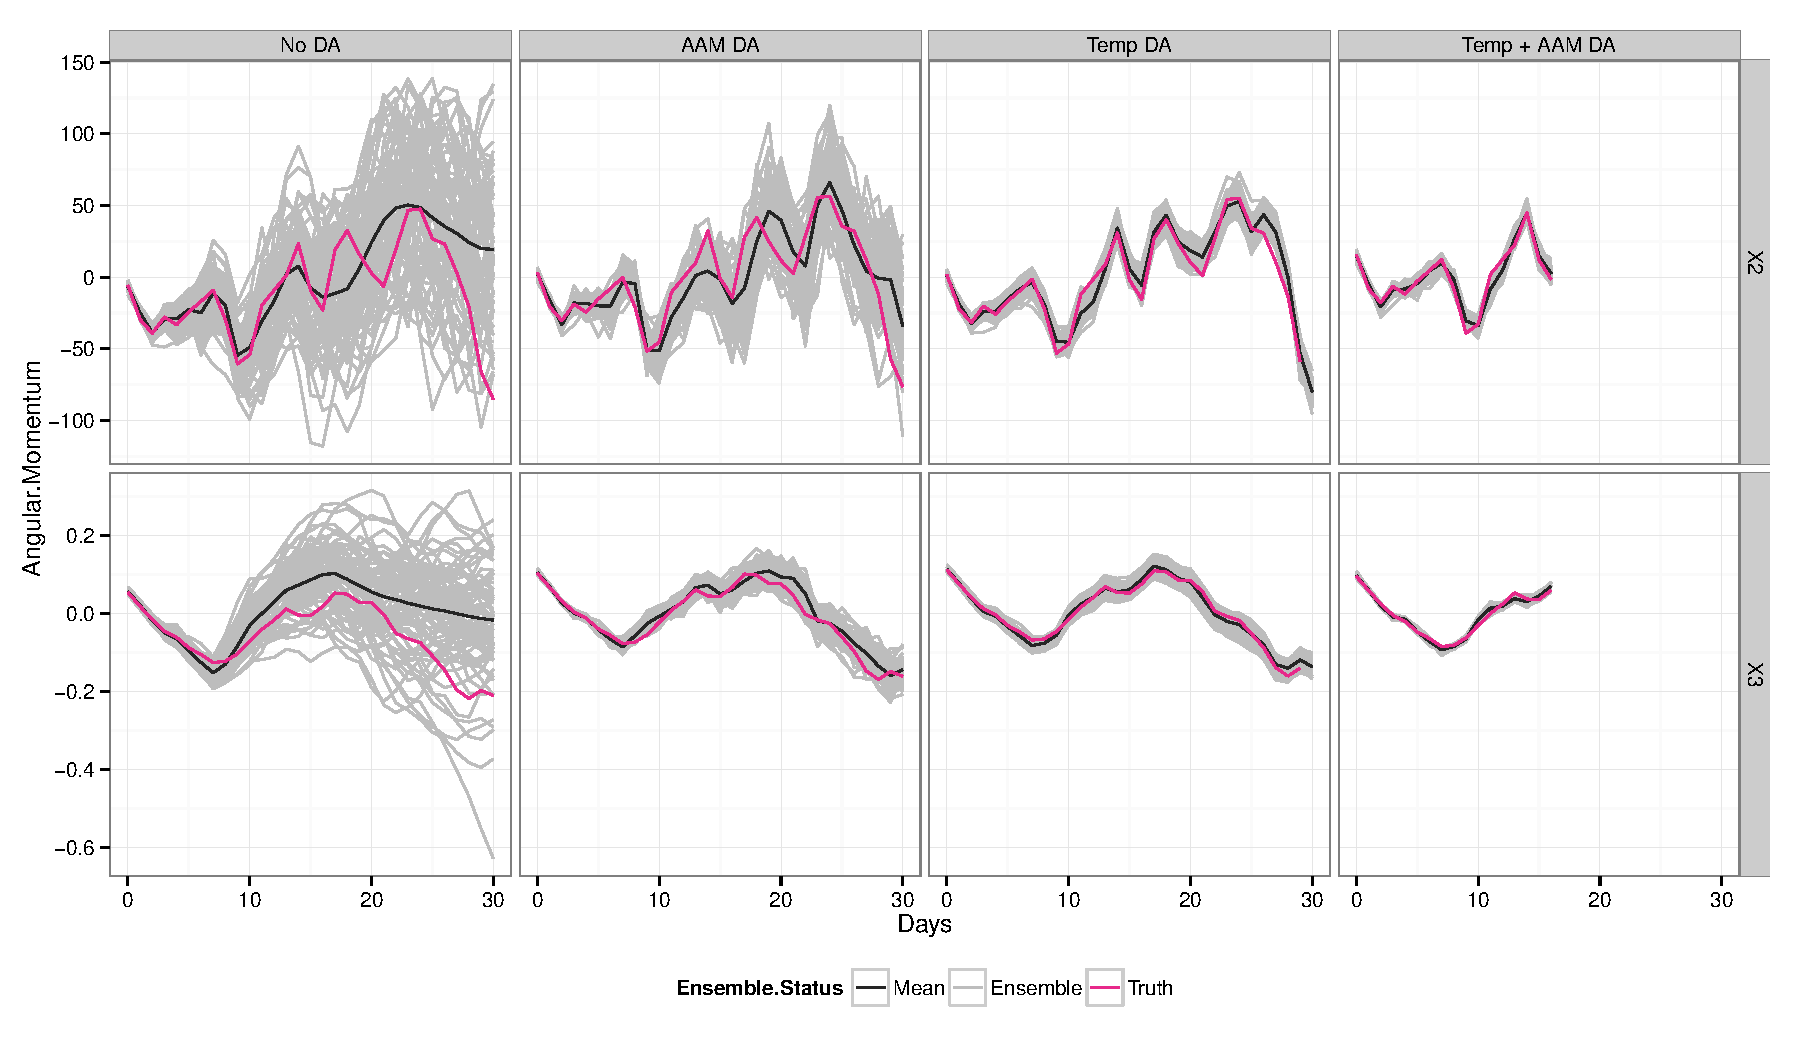
\includegraphics[width=\textwidth]{Paper_figures/ERPDA_paper_erpda_obs_space.pdf} 
\caption{ The DART-CAM prior ensemble (gray) and its mean (black) compared to the true state (pink) in terms of angular momentum components $\chi_2$ and $\chi_3$, comparing four perfect-model experiments with DART-CAM (see text and Table \ref{tab:expts}).  }
 \label{fig:fit_to_ERPs}
\end{figure}

%-----evolution of the covariances between local variables and the AAM observations 
 \begin{figure}
	 \includegraphics[width=\textwidth]{Paper_figures/ERPDA_paper_U_to_LOD_covariances.pdf}
	 \caption{Snapshots of the covariance between the zonal wind and the axial angular momentum ($\chi_3$) shortly after spin-up (top row), at the end of the assimilation period (middle row), and averaging over the entire period minus spinup time (bottom row), assimilatng only the angular momentum. The lefthand column shows snapshots at 320 hPa; the righthand column shows snapshots at 10 hPa.}
 \label{fig:covariances}
\end{figure}

%-----evolution of the prior error and corresponding increments 
 \begin{figure}
	 \includegraphics[height=0.9\textheight]{Paper_figures/ERPDA_paper_U_priorerror_vs_increment_vs_ER_30jan_strattrop.pdf}
	 \caption{Snapshots of the 320 hPa zonal wind (a) true error (true minus prior ensemble mean), (b) analysis increment (posterior minus prior ensemble mean), (c) square error reduction (posterior minus prior mean square error), and (d) variance reduction (posterior minus prior ensemble variance, scaled as in (\ref{eq:EvsS})). All plots are shown for 30 Jan, for the CAM ensemble assimilating only atmospheric angular momentum. } 
 \label{fig:error_increments}
\end{figure}

%-----focus on the ensemble in two regions to show how it is moved away from the true state
 \begin{figure}
	 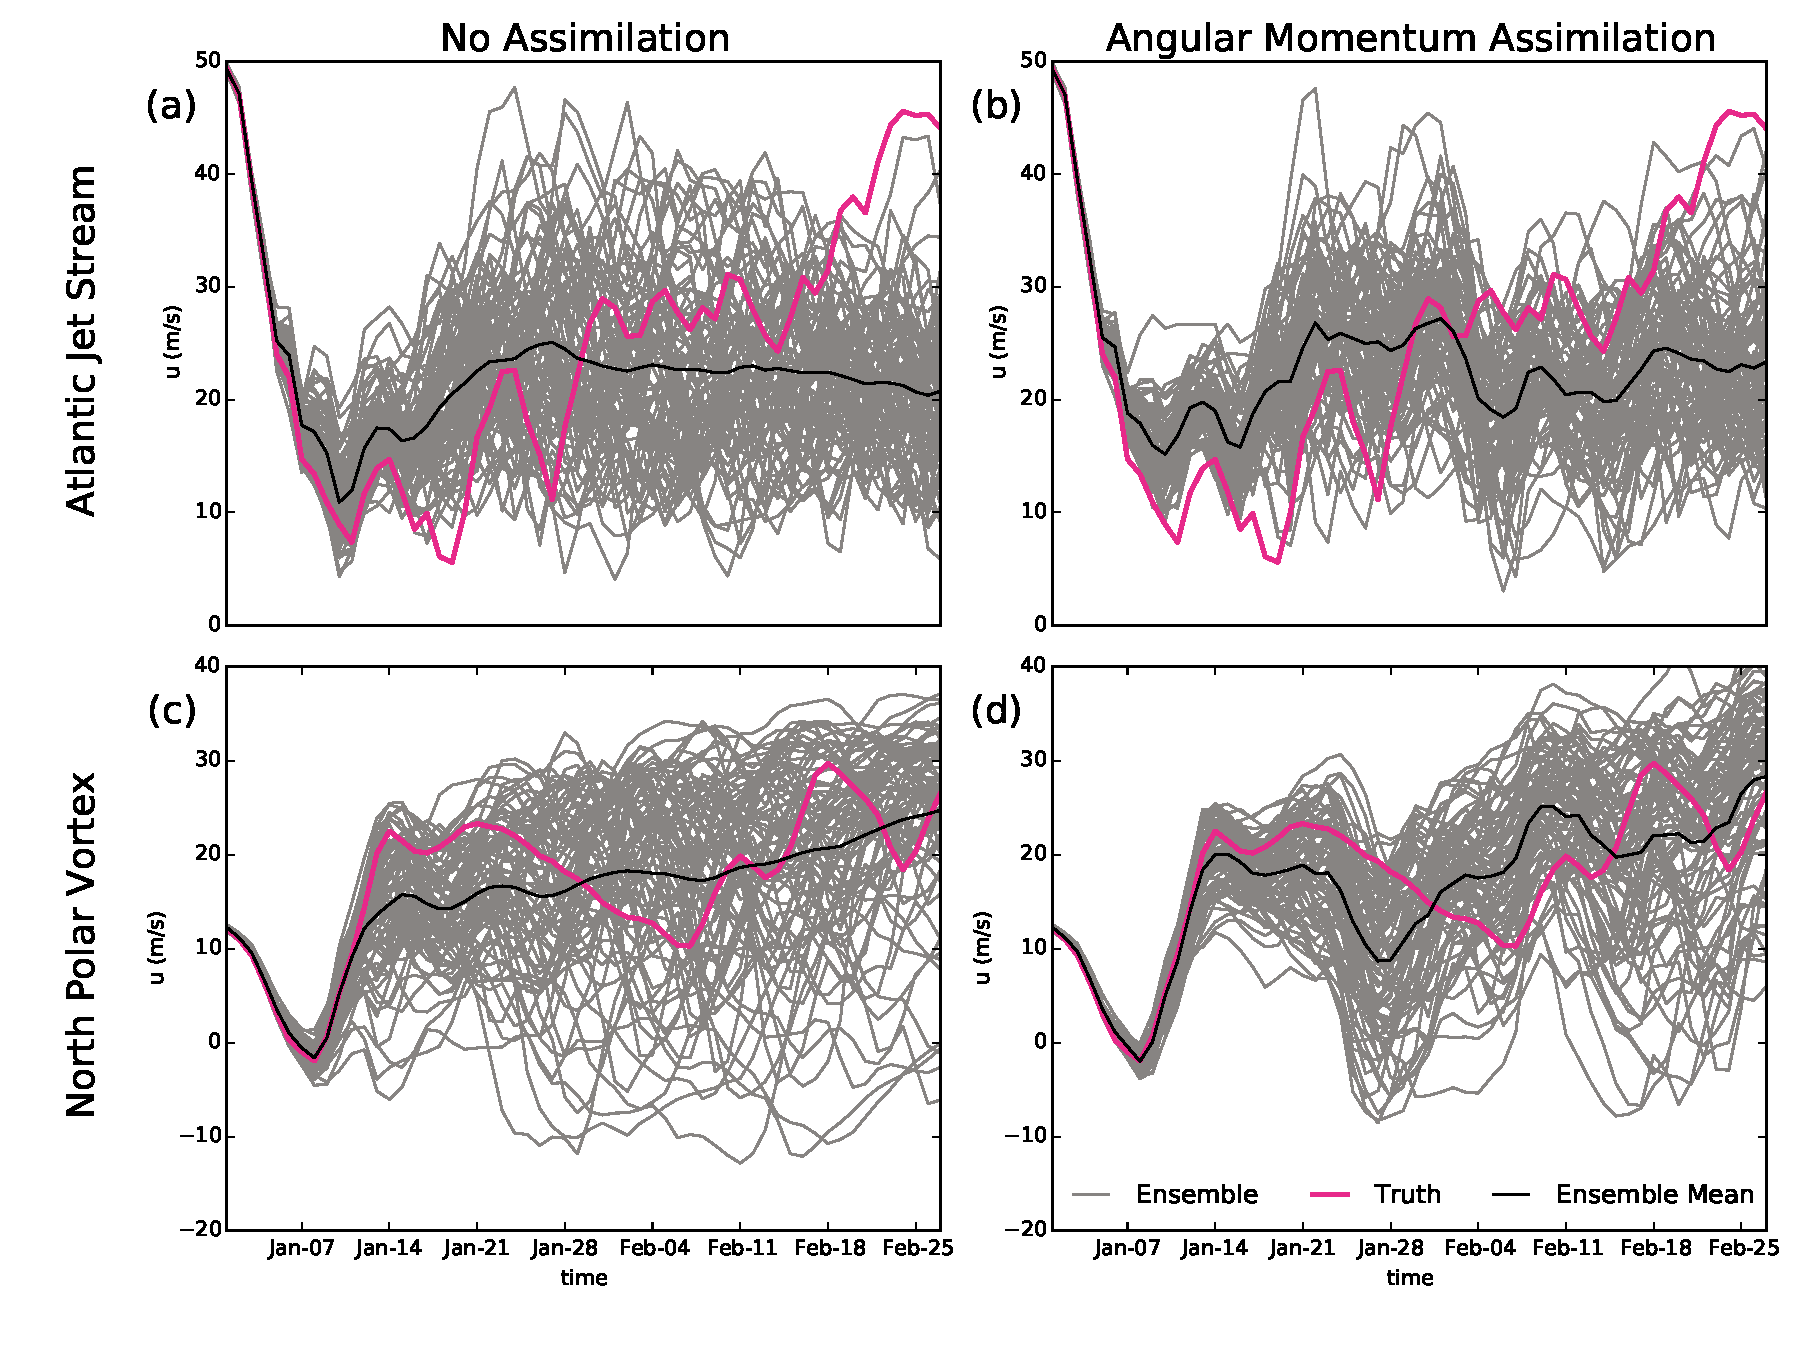
\includegraphics[width=\textwidth]{Paper_figures/ERPDA_paper_point_checks.pdf}
	 \caption{Comparison of the ensemble and its mean to the true state, comparing no assimilation (left column), and assimilation of the three angular momentum components (right column). The top row shows zonal wind averaged over the Atlantic jet stream, and the bottom row shows zonal wind averaged in the polar vortex (see text).}
	 \label{fig:point_checks}
\end{figure}


%------MSE diff between ERPRST and RST (red is good)
 \begin{figure}
	 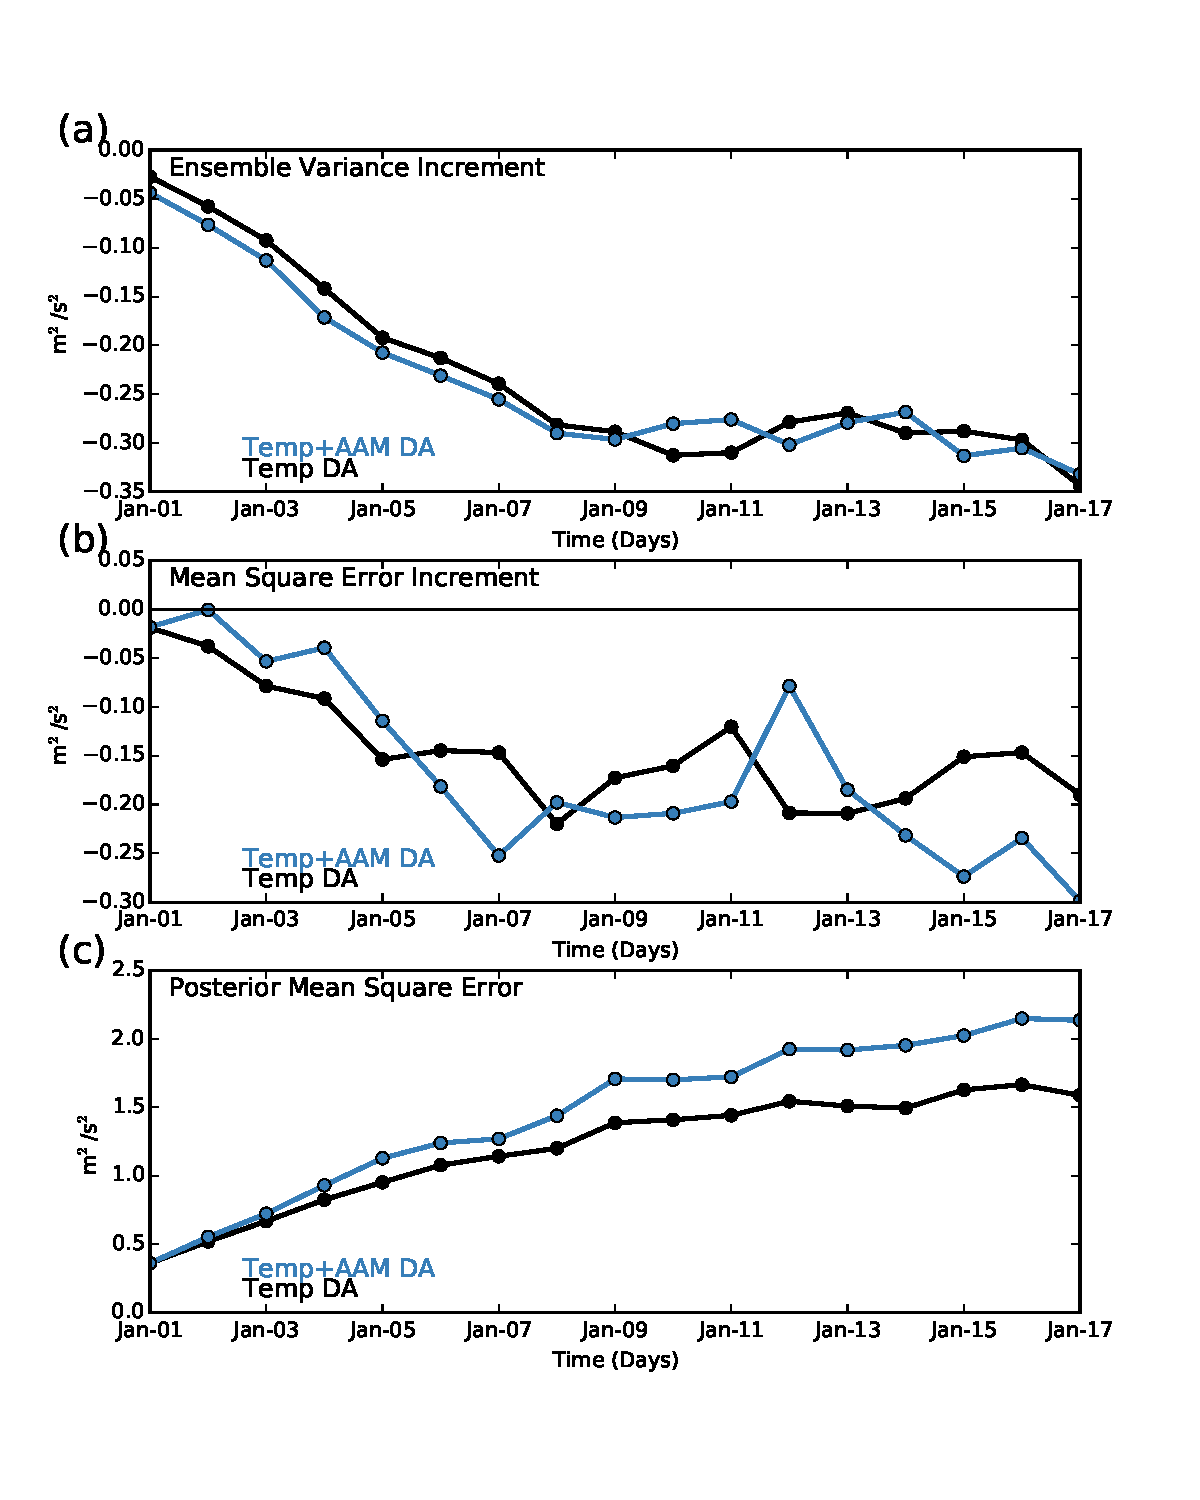
\includegraphics[width=0.7\textwidth]{Paper_figures/ERPDA_paper_MSE_RST_vs_ERPRST_global.pdf}
	 \caption{(a) Global average increment (posterior-prior) in the ensemble variance, scaled as in (\ref{eq:EvsS}), for zonal wind in a DART-WACCM ensemble assimilating local temperatures (black) and temperatures along with atmospheric angular momentum (blue). (b) As in (a), but for the increment in the mean square error. (c) As above, but showing the absolute posterior mean square error.}
	 \label{fig:added_value_MSE}
\end{figure}

%-------comparison of the WACCM experiments in terms of true error ----
 \begin{figure}
	 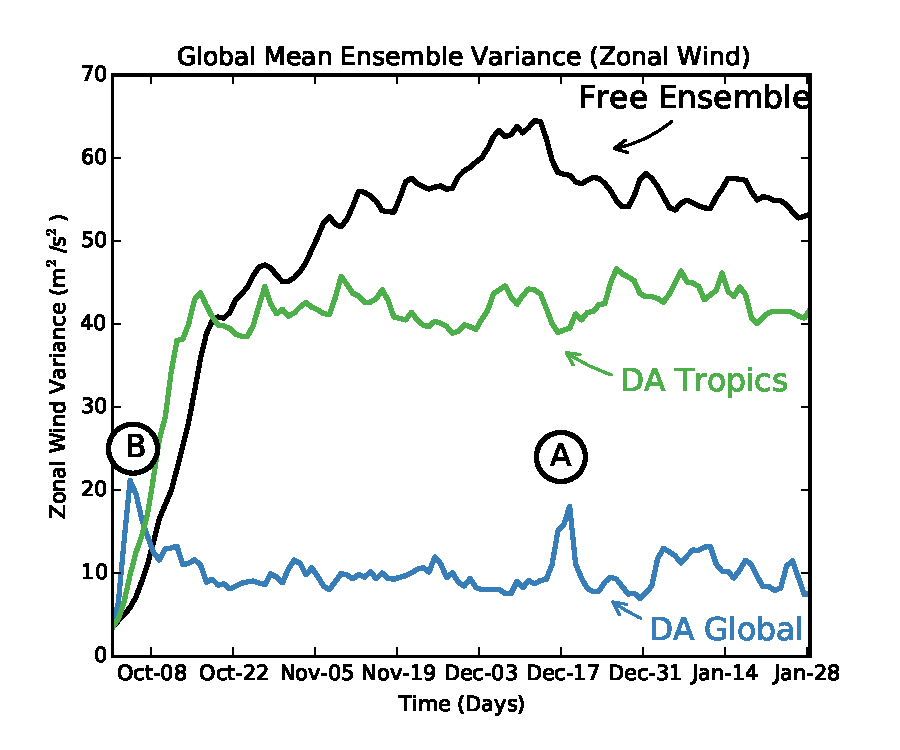
\includegraphics[width=\textwidth]{Paper_figures/ERPDA_paper_evalvariable_state_space.pdf}
	 \caption{Global-average ensemble variance in the zonal wind as a function of time, comparing a DART-WACCM with no assimilation, and with 6-hourly assimilation of meteorolgical observations (see text).}
	 \label{fig:evalvariable_state}
\end{figure}
%-------comparison of the WACCM experiments in terms of aam ----
\begin{figure}
	 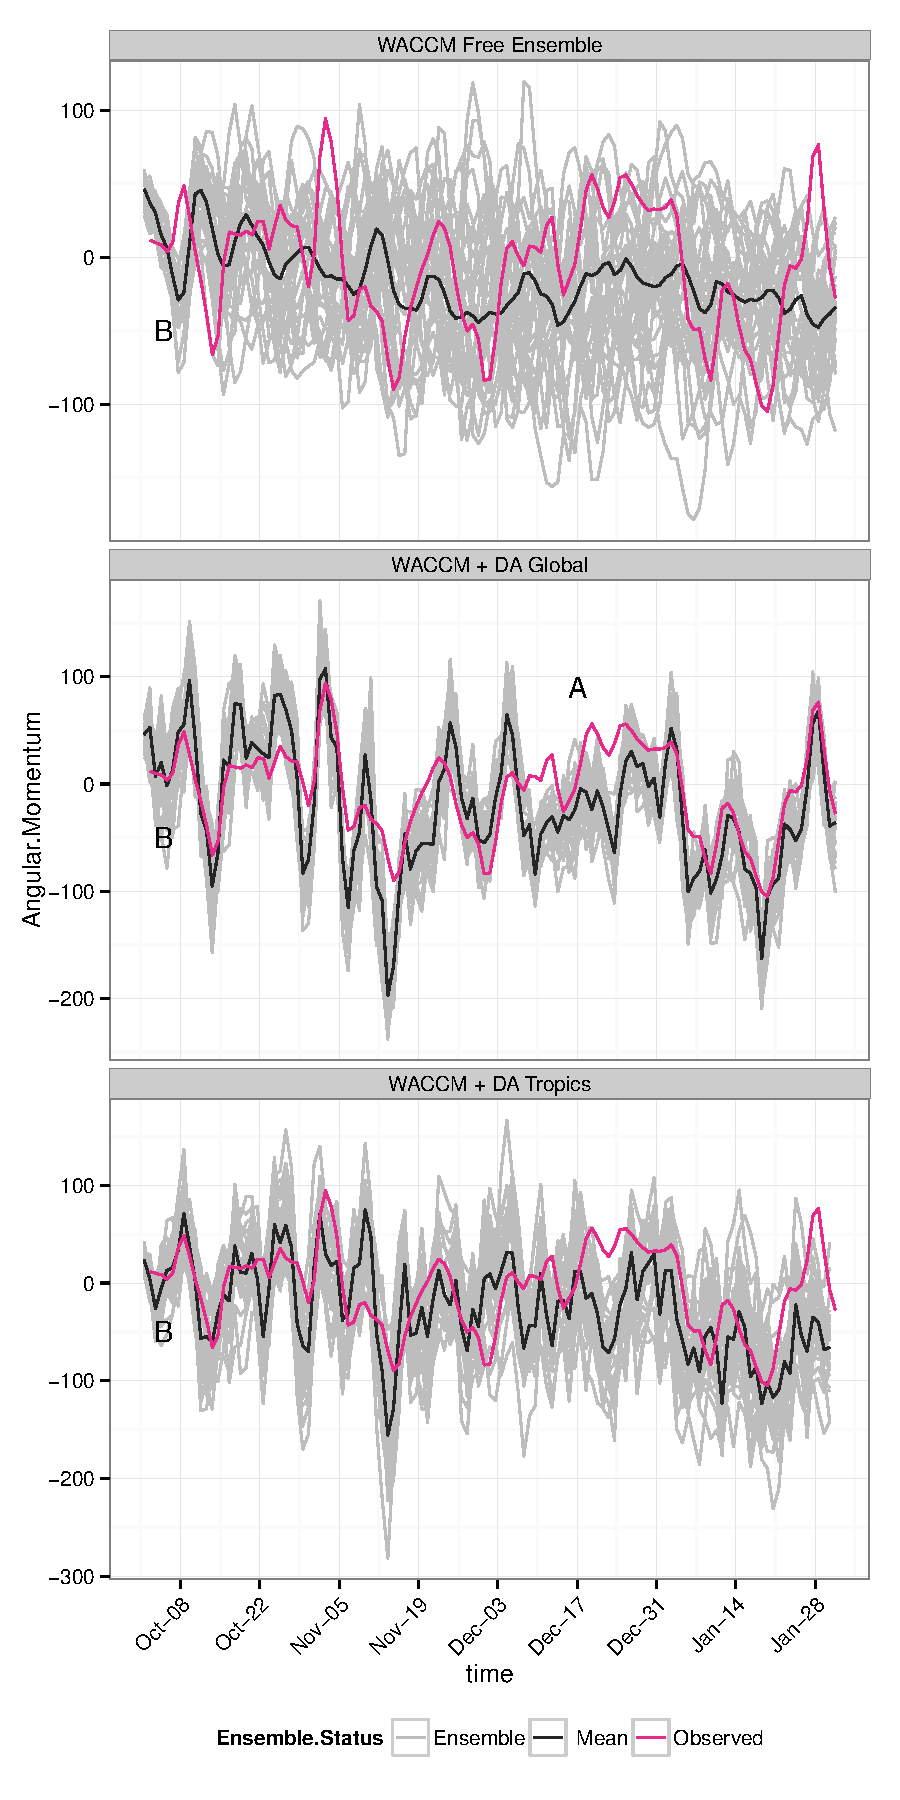
\includegraphics[width=0.5\textwidth]{Paper_figures/ERPDA_paper_evalvariable_aam_space_X2only.pdf}
	 \caption{Comparison of the ensemble (gray) and its mean (black) in DART-WACCM experiments with increasing observational constraints (Table \ref{tab:expts}), in terms of angular momentum excitation functions $\chi_2$ and $\chi_3$ Each angular momentum function is compared to the angular momentum implied by the corresponding Earth rotation parameters (pink).}
	 \label{fig:evalvariable_aam}
\end{figure}



% DO NOT USE \psfrag or \subfigure commands.
%
% Figure captions go below the figure.
% Table titles go above tables; all other caption information
%  should be placed in footnotes below the table.
%
%----------------
% EXAMPLE FIGURE
%
% \begin{figure}
% \noindent\includegraphics[width=20pc]{samplefigure.eps}
% \caption{Caption text here}
% \label{figure_label}
% \end{figure}
%
% ---------------
% EXAMPLE TABLE
%
%\begin{table}
%\caption{Time of the Transition Between Phase 1 and Phase 2\tablenotemark{a}}
%\centering
%\begin{tabular}{l c}
%\hline
% Run  & Time (min)  \\
%\hline
%  $l1$  & 260   \\
%  $l2$  & 300   \\
%  $l3$  & 340   \\
%  $h1$  & 270   \\
%  $h2$  & 250   \\
%  $h3$  & 380   \\
%  $r1$  & 370   \\
%  $r2$  & 390   \\
%\hline
%\end{tabular}
%\tablenotetext{a}{Footnote text here.}
%\end{table}

% See below for how to make sideways figures or tables.

\end{document}

%%%%%%%%%%%%%%%%%%%%%%%%%%%%%%%%%%%%%%%%%%%%%%%%%%%%%%%%%%%%%%%

More Information and Advice:

%% ------------------------------------------------------------------------ %%
%
%  SECTION HEADS
%
%% ------------------------------------------------------------------------ %%

% Capitalize the first letter of each word (except for
% prepositions, conjunctions, and articles that are
% three or fewer letters).

% AGU follows standard outline style; therefore, there cannot be a section 1 without
% a section 2, or a section 2.3.1 without a section 2.3.2.
% Please make sure your section numbers are balanced.
% ---------------
% Level 1 head
%
% Use the \section{} command to identify level 1 heads;
% type the appropriate head wording between the curly
% brackets, as shown below.
%
%An example:
%\section{Level 1 Head: Introduction}
%
% ---------------
% Level 2 head
%
% Use the \subsection{} command to identify level 2 heads.
%An example:
%\subsection{Level 2 Head}
%
% ---------------
% Level 3 head
%
% Use the \subsubsection{} command to identify level 3 heads
%An example:
%\subsubsection{Level 3 Head}
%
%---------------
% Level 4 head
%
% Use the \subsubsubsection{} command to identify level 3 heads
% An example:
%\subsubsubsection{Level 4 Head} An example.
%
%% ------------------------------------------------------------------------ %%
%
%  IN-TEXT LISTS
%
%% ------------------------------------------------------------------------ %%
%
% Do not use bulleted lists; enumerated lists are okay.
% \begin{enumerate}
% \item
% \item
% \item
% \end{enumerate}
%
%% ------------------------------------------------------------------------ %%
%
%  EQUATIONS
%
%% ------------------------------------------------------------------------ %%

% Single-line equations are centered.
% Equation arrays will appear left-aligned.

Math coded inside display math mode \[ ...\]
 will not be numbered, e.g.,:
 \[ x^2=y^2 + z^2\]

 Math coded inside \begin{equation} and \end{equation} will
 be automatically numbered, e.g.,:
 \begin{equation}
 x^2=y^2 + z^2
 \end{equation}

% IF YOU HAVE MULTI-LINE EQUATIONS, PLEASE
% BREAK THE EQUATIONS INTO TWO OR MORE LINES
% OF SINGLE COLUMN WIDTH (20 pc, 8.3 cm)
% using double backslashes (\\).

% To create multiline equations, use the
% \begin{eqnarray} and \end{eqnarray} environment
% as demonstrated below.
\begin{eqnarray}
  x_{1} & = & (x - x_{0}) \cos \Theta \nonumber \\
        && + (y - y_{0}) \sin \Theta  \nonumber \\
  y_{1} & = & -(x - x_{0}) \sin \Theta \nonumber \\
        && + (y - y_{0}) \cos \Theta.
\end{eqnarray}

%If you don't want an equation number, use the star form:
%\begin{eqnarray*}...\end{eqnarray*}

% Break each line at a sign of operation
% (+, -, etc.) if possible, with the sign of operation
% on the new line.

% Indent second and subsequent lines to align with
% the first character following the equal sign on the
% first line.

% Use an \hspace{} command to insert horizontal space
% into your equation if necessary. Place an appropriate
% unit of measure between the curly braces, e.g.
% \hspace{1in}; you may have to experiment to achieve
% the correct amount of space.


%% ------------------------------------------------------------------------ %%
%
%  EQUATION NUMBERING: COUNTER
%
%% ------------------------------------------------------------------------ %%

% You may change equation numbering by resetting
% the equation counter or by explicitly numbering
% an equation.

% To explicitly number an equation, type \eqnum{}
% (with the desired number between the brackets)
% after the \begin{equation} or \begin{eqnarray}
% command.  The \eqnum{} command will affect only
% the equation it appears with; LaTeX will number
% any equations appearing later in the manuscript
% according to the equation counter.
%

% If you have a multiline equation that needs only
% one equation number, use a \nonumber command in
% front of the double backslashes (\\) as shown in
% the multiline equation above.

%% ------------------------------------------------------------------------ %%
%
%  SIDEWAYS FIGURE AND TABLE EXAMPLES
%
%% ------------------------------------------------------------------------ %%
%
% For tables and figures, add \usepackage{rotating} to the paper and add the rotating.sty file to the folder.
% AGU prefers the use of {sidewaystable} over {landscapetable} as it causes fewer problems.
%
% \begin{sidewaysfigure}
% \includegraphics[width=20pc]{samplefigure.eps}
% \caption{caption here}
% \label{label_here}
% \end{sidewaysfigure}
%
%
%
% \begin{sidewaystable}
% \caption{}
% \begin{tabular}
% Table layout here.
% \end{tabular}
% \end{sidewaystable}
%
%

